
\documentclass[12pt]{article}

\usepackage{amsmath,amsthm,amssymb}
\usepackage{graphicx}

\newcommand{\C}{\mathbb{C}}
\newcommand{\Z}{\mathbb{Z}}
\renewcommand{\Im}{\text{Im}}
\renewcommand{\Re}{\text{Re}}

\begin{document}

\title{Hw. 1 Problem 2}
\maketitle


The 6th roots of unity areall the complex solutions, $z$, to $z^6-1=0$, or equivalently, $z^6= 1 = e^{i0}$. Any such solution can be uniquely written as $$e^{i(0+{2\pi k\over 6})}= e^{i{\pi\over3}k}$$
When $k\in \Z, 0\le k < 6$. The 6th roots of unity are therefore,

\begin{align*}
e^{i0}&=1,\\
e^{i{\pi\over3}}&=\cos {\pi\over 3} + i\sin{\pi\over 3} = {1\over2}+i{\sqrt{3}\over2},\\ 
e^{i{2\pi\over3}}&=\cos {2\pi\over 3} + i\sin{2\pi\over 3} = -{1\over2}+i{\sqrt{3}\over2},\\
e^{i{3\pi\over3}}&=e^{i\pi}=\cos {\pi} + i\sin{\pi} = -1,\\
e^{i{4\pi\over3}}&=\cos {4\pi\over 3} + i\sin{4\pi\over 3} = -{1\over2}-i{\sqrt{3}\over2},\\
e^{i{5\pi\over3}}&=\cos {5\pi\over 3} + i\sin{5\pi\over 3} = {1\over2}-i{\sqrt{3}\over2}.
\end{align*}

\newpage
Graph:

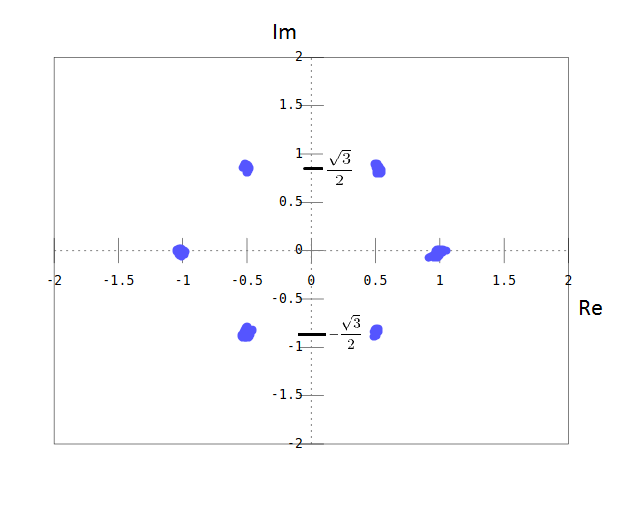
\includegraphics[scale=0.8]{q2}


\end{document}
